\documentclass[11pt]{article}
\usepackage[T1]{fontenc}
\usepackage{lmodern}
\usepackage[margin=1in]{geometry}
\usepackage{amsmath,amssymb,amsthm,mathtools}
\usepackage{microtype}
\usepackage{booktabs,array,enumitem}
\usepackage{xcolor,tikz}
\usetikzlibrary{arrows.meta,positioning,calc,patterns}
\usepackage[hyphens]{url}
\usepackage[colorlinks=true,linkcolor=blue!45!black,citecolor=blue!45!black,urlcolor=blue!45!black]{hyperref}
\numberwithin{equation}{section}
\newtheorem{theorem}{Theorem}[section]
\newtheorem{proposition}[theorem]{Proposition}
\newtheorem{lemma}[theorem]{Lemma}
\newtheorem{corollary}[theorem]{Corollary}
\theoremstyle{definition}
\newtheorem{definition}[theorem]{Definition}
\theoremstyle{remark}
\newtheorem{remark}[theorem]{Remark}
\newcommand{\R}{\mathbb R}
\newcommand{\C}{\mathbb C}
\newcommand{\Z}{\mathbb Z}
\newcommand{\N}{\mathbb N}
\newcommand{\E}{\mathbb E}
\newcommand{\Prob}{\mathbb P}
\newcommand{\one}{\mathbf 1}
\newcommand{\inner}[2]{\langle #1,#2\rangle}
\newcommand{\norm}[1]{\lVert #1\rVert}
\DeclareMathOperator{\supp}{supp}
\DeclareMathOperator{\Tr}{Tr}
\DeclareMathOperator{\Cov}{Cov}
\DeclareMathOperator{\sgn}{sgn}
\setlist[enumerate]{leftmargin=*,itemsep=0.3em}
\setlength{\emergencystretch}{2em}
\allowdisplaybreaks[2]

\hypersetup{pdftitle={An Isolated Particle Pole for the Two-Dimensional O(3) Spin Field},pdfauthor={OpenAI},bookmarksnumbered=true}
\title{An Isolated Particle Pole for the\protect\\ Two-Dimensional $O(3)$ Spin Field}
\author{OpenAI}
\date{October 4, 2026}
\begin{document}
\maketitle
\begin{abstract}
We consider the continuum spin field constructed from the nearest-neighbor
two-dimensional $O(3)$ model by the fixed prescription of the companion
paper. We prove that its vector two-point spectral measure has a positive
atom corresponding to the lowest mass, separated by a positive gap from
all remaining mass support.
\end{abstract}
\setcounter{tocdepth}{1}
\tableofcontents
\clearpage
\section{Introduction}
\label{sec:introduction}

A mass gap and an isolated particle mass are different spectral statements.
A positive spectral measure may start at a strictly positive threshold and
still have no atoms. For the spin field of the two-dimensional $O(3)$ model,
we prove that the lowest mass is an atom separated from all remaining mass
support. The proof uses the massive continuum construction in
\cite{OpenAI-O3}, including its uniform finite-volume estimates.

\subsection{The field and the result}

Let $\phi=(\phi^1,\phi^2,\phi^3)$ be the Hermitian vector field obtained
from the nearest-neighbor $O(3)$ model by the fixed lattice-spacing and
field-normalization prescription of \cite[Theorem~1.2]{OpenAI-O3}.
Here the Euclidean lattice is two-dimensional and the reconstructed
spacetime has one time and one space dimension. Internal $O(3)$ symmetry
and the K\"all\'en--Lehmann representation give
\begin{equation}
 W_2^{ij}(x)=\delta_{ij}\int_{[0,\infty)}
       \Delta_+(x;\mu^2)\,\rho(d\mu^2),
 \label{intro:spectral}
\end{equation}
where $\Delta_+(x;\mu^2)$ is the positive-frequency free scalar
two-point distribution and $\rho$ is a positive measure. The variable
$\mu$ denotes mass; the argument of $\rho$ is mass squared. This
representation records the masses to which the field couples
\cite{Kallen1952,Lehmann1954}.

\begin{theorem}[An isolated lowest mass]
\label{intro:main}
For the field $\phi$ just specified, there exist $m_1,Z,\delta>0$ and a
positive measure $\rho_{\mathrm{rest}}$ such that
\begin{equation}
 \rho=Z\delta_{m_1^2}+\rho_{\mathrm{rest}},
 \qquad
 \supp\rho_{\mathrm{rest}}\subset[(m_1+\delta)^2,\infty).
 \label{intro:atom}
\end{equation}
In particular, $m_1$ is the smallest mass in the support of the spin-field
two-point function.
\end{theorem}

The atom in \eqref{intro:atom} is the isolated particle contribution
to the two-point function. Both its positive weight and its separation
from the remaining spectrum must be established: neither follows from
exponential decay alone. Our use of the continuum construction is made
precise in Section~\ref{sec:inputs}. The new argument begins with its
uniform torus estimates and does not assume that an eigenvalue at finite
circumference persists in the infinite-volume limit.

\subsection{Context and methods}

The two-dimensional nonlinear sigma models are basic examples in which
short-distance behavior and massive long-distance behavior must be
reconciled. Polyakov's work on the interaction of Goldstone particles
identified the role of asymptotic freedom in these models
\cite{Polyakov1975}. The factorized scattering description of the
$O(N)$ sigma model developed by Zamolodchikov and Zamolodchikov gives
a particle-based account of its expected massive continuum physics
\cite{Zamolodchikov1979}. Relating such a description to the field
obtained from a specified lattice limit requires control of that limit
and of the field's spectral measure. Within the massive-particle
description, Balog and Niedermaier computed spin-field form factors and
spectral densities \cite{BalogNiedermaier1997}. The present argument
establishes the isolated mass directly for the field obtained from the
lattice prescription.

In constructive field theory, Glimm, Jaffe, and Spencer proved an
isolated particle mass for weakly coupled $P(\phi)_2$ models by a
particle cluster expansion \cite{GlimmJaffeSpencer1974}. The setting
and the estimates used here are different: our starting point is the
finite-volume control accompanying the $O(3)$ lattice limit.

The companion construction \cite{OpenAI-O3} provides the continuum
field, its Osterwalder--Schrader reconstruction
\cite{OsterwalderSchrader1973,OsterwalderSchrader1975}, a gap above the
vacuum, and a nonzero one-field state. It also supplies two inputs that
are decisive here: exponentially small partition-function defects under
doubling of large physical squares, uniformly in the lattice cutoff,
and uniform factorial moment bounds for normalized local spin sums.
We use these quantitative estimates to extract the isolated mass.

Several classical correlation tools enter the passage from transfer
energies to field correlations. The positivity arguments belong to the
Griffiths--Ginibre theory and its extensions to multicomponent rotators
\cite{Ginibre1970,Dunlop1976}. We give the particular three-component
argument in full, because it must control arbitrary spin polynomials
invariant under simultaneous spin inversion. Positive association
\cite{FKG1971} and the
Edwards--Sokal coupling \cite{EdwardsSokal1988} relate spin correlations
to connection events for embedded Ising signs.
The crossing theorem of K\"ohler-Schindler and Tassion
\cite{KohlerSchindlerTassion2023} supplies circuits using only symmetry
and positive association. These circuits attach a definite amount of
normalized spin-field weight to connections; the normalization is
essential as the lattice spacing tends to zero.

The use of bounded-energy state counts to constrain particle content is
related to the phase-space criteria of Haag and Swieca
\cite{HaagSwieca1965} and Buchholz and Wichmann
\cite{BuchholzWichmann1986}. Here the needed estimate is obtained directly
from finite-volume transfer traces. Testing an interval of momenta then
constrains the mass support without presupposing that its points are atoms.

\subsection{Proof strategy}

Write $m_*$ for the bottom of the mass support of $\rho$; the source
gap and nonzero one-field norm imply $0<m_*<\infty$. At lattice cutoff
$N$ and spatial circumference $w$, let $e_N(w)$ be the least positive
transfer energy, and let $\mathcal N_{N,w}(u)$ count all transfer
energies at most $u$, with multiplicity and with the vacuum included.
The proof first compares $e_N(w)$ with $m_*$, then bounds the number
of low transfer energies and uses that bound to constrain the mass support.

\begin{enumerate}
\item Section~\ref{sec:transfer} derives rectangular trace bounds and
local torus-to-plane comparison from the square partition-function
input. This also gives a positive lower bound for $e_N(w)$, uniform
in the cutoff and in sufficiently large circumferences.

\item Section~\ref{sec:parity} bounds covariances of even spin
polynomials by the square of a two-point correlation. Consequently,
among row functions unchanged by simultaneous spin inversion, every
nonvacuum transfer energy is at least $2e_N(w)$.
The lowest excitation is odd, with a quantitative overlap
that allows its sign to be tested by spin clusters.

\item Section~\ref{sec:visibility} combines those clusters with local
circuits to prove
\[
 \liminf_{w\to\infty}\liminf_{N\to\infty}e_N(w)\ge m_*.
\]
Here and in the counting step, $w$ runs through a fixed dyadic sequence
of physical circumferences. This comparison identifies the mass scale
needed for counting, without selecting a limiting eigenvector.

\item Section~\ref{sec:counting} proves
\[
 \limsup_{N\to\infty}\mathcal N_{N,w}(3m_*/2)\le Cw.
\]
Exchanging the directions of a torus compares the heat trace at
circumference $2w$ with the square of the trace at circumference $w$.
A positive polynomial approximation to an energy cutoff shows that,
below the two-excitation threshold, doubling the circumference can at
most double the count, up to summable errors.

\item Section~\ref{sec:mass-support} uses spatial momentum projections
and convergence of smeared two-point functions to show that $J$
distinct masses near $m_*$ require at least $cJw$ such states. The
constant $c>0$ is independent of $J$. Hence there are only finitely
many masses near $m_*$, and their smallest point is the atom in
Theorem~\ref{intro:main}.
\end{enumerate}

Throughout, cutoff limits are taken at fixed physical circumference
before that circumference tends to infinity. The trace and moment
estimates permit the comparisons needed in this order.

\section{The continuum field and the uniform lattice inputs}
\label{sec:inputs}

We first specify the construction used in this paper and the estimates
we retain from it.  The finite-volume estimates are essential: a gap in
the continuum Hamiltonian alone would not control how many transfer
states can approach its lower edge.

Let $\sigma$ be normalized area measure on $S^2$.  At cutoff $N$, the
lattice spacing is $a=a_N=L^{-N}$, and the probability on a periodic
nearest-neighbor lattice $\Lambda$ is
\begin{equation}
 d\mu_{N,\Lambda}(q)
 =Z_{N,\Lambda}^{-1}
   \exp\!\left(\beta_N\sum_{\{x,y\}\in E(\Lambda)}q_x\cdot q_y\right)
   \prod_{x\in\Lambda}d\sigma(q_x).
 \label{inp:lattice}
\end{equation}
Each bond occurs once; there is no external field.  We use the fixed
prescription of \cite[Theorem~1.2]{OpenAI-O3}: $L$ is a fixed dyadic
integer, the terminal coupling $H$ is sufficiently large, and
\[
 \beta_N=H+\frac{\log L}{2\pi}N+O(\log(N+1)),\qquad B_N>0.
\]
The positive field normalization $B_N$ is the one in that prescription.
For a real test $f\in C_c^\infty(\R^2)$ and a component $i$, put
\begin{equation}
 X_f^i=B_Na^2\sum_x f(x)q_x^i.
 \label{inp:field}
\end{equation}
Coordinates $x$ and all torus lengths are physical.  Torus tests are
periodized from their indicated local charts.  The cutoff plane state
is the limit of periodic square tori, as in
\cite[Proposition~2.1]{OpenAI-O3}; no boundary spins are fixed.
For time reflection, write $(\theta f)(t,b)=f(-t,b)$.

Here are the precise construction results needed below.  They hold for
this same trajectory, normalization, and periodic state.

\begin{proposition}[Inputs from the continuum construction]
\label{inp:contracts}
There are integers $K_0,M_0>0$ and constants $c,C>0$ with the following
properties.  Write $w_k=M_0 2^k$, and let $Z_N(t,w)$ be the partition
function on a torus of time length $t$ and spatial circumference $w$.
\begin{enumerate}[label=\textup{(\roman*)}]
\item In the cutoff plane, all joint moments of the variables
\eqref{inp:field} converge to those of the Euclidean field $\phi$.
The limiting Schwinger distributions are tempered, Euclidean invariant,
and $O(3)$ covariant.  Their Osterwalder--Schrader reconstruction is the
Wightman field of Theorem~\ref{intro:main}, with unique vacuum $\Omega$
and
\[
 H_{\mathrm{phys}}|_{\Omega^\perp}\ge m>0.
\]
For some real test $f$ supported strictly in positive time, the
one-field reflection norm
$\E[\phi^1(\theta f)\phi^1(f)]$ is strictly positive.
\item For all $N\ge K_0$ and $k\ge0$,
\begin{equation}
 0\le \Delta_N(w_k)
 :=4\log Z_N(w_k,w_k)-\log Z_N(2w_k,2w_k)
 \le C e^{-c w_k}.
 \label{inp:defect}
\end{equation}
\item On these square tori and on the cutoff plane, the component
moment measures
\[
 S_{r,N}^{\boldsymbol i}
 =(B_Na^2)^r\sum_{x_1,\ldots,x_r}
     \E\!\left[\prod_{j=1}^r q_{x_j}^{i_j}\right]
     \delta_{(x_1,\ldots,x_r)}
\]
are nonnegative.  For arbitrary translated unit boxes $Q_1,\ldots,Q_r$,
\begin{equation}
 S_{r,N}^{\boldsymbol i}(Q_1\times\cdots\times Q_r)
 \le C^r r!,
 \label{inp:majorant}
\end{equation}
uniformly in $N\ge K_0$, the square torus, the box positions, and the
component indices.
\end{enumerate}
\end{proposition}

For completeness, the source locators distinguish the different
strengths of these inputs.  Part~(i) uses
\cite[Propositions~10.2, 10.3, 11.3, and 11.4]{OpenAI-O3}; the nonzero
one-field norm is proved in the final paragraph of the proof of
Proposition~11.5.  The reconstruction and separated-time
Euclidean continuation are those of
Osterwalder and Schrader~\cite{OsterwalderSchrader1973,OsterwalderSchrader1975}.
Part~(ii) follows from the uniform reference-box test and rectangular
doubling criterion in \cite[Propositions~8.1 and 8.3]{OpenAI-O3}:
the base defect is at most $2^{-10}$ and the defect after $k$ doublings
is at most $64^{-1}2^{-2^k}$.  Their application to the constructed
trajectory is made in \cite[Theorem~8.4]{OpenAI-O3}.  Part~(iii) is
\cite[Proposition~10.1]{OpenAI-O3}.  These statements retain the
fixed parameter choices of that construction, including sufficiently
large $H$.

\subsection{The bottom of the two-point mass support}

Let $\rho$ be the positive spectral measure in
\eqref{intro:spectral}, and define
\[
 \mathcal M=\{\sqrt{s}:s\in\supp\rho\},\qquad m_*=\inf\mathcal M.
\]
The following consequences do not presume that $\rho$ has an atom.

\begin{lemma}[Positive massive Euclidean kernel]
\label{inp:kernel}
One has $0<m_*<\infty$.  At separated Euclidean points, the
like-component two-point function is the continuous kernel
\begin{equation}
 C(t,b)=\int\rho(d\mu^2)\int_{\R}\frac{dp}{2\pi}
          \frac{e^{ipb-tE(p,\mu)}}{2E(p,\mu)},
 \qquad E(p,\mu)=\sqrt{p^2+\mu^2},\quad t>0.
 \label{inp:euclidean}
\end{equation}
It is strictly positive at every nonzero Euclidean separation, and
there is a constant $C_0$ such that
\begin{equation}
 0<C(t,b)\le C_0e^{-m_*\sqrt{t^2+b^2}}
 \quad\text{when }\sqrt{t^2+b^2}\ge1.
 \label{inp:decay}
\end{equation}
\end{lemma}

\begin{proof}
Internal symmetry gives $\E\phi^i(f)=0$, so one-field vectors lie in
$\Omega^\perp$.  Their positive energy-momentum spectral measures
therefore put no weight at energies in $[0,m)$.  If $\supp\rho$ met
$(0,m^2)$, some compact interval $J\subset(0,m^2)$ would have positive
$\rho$-measure.  At sufficiently small spatial momenta, all shells
with mass squared in $J$ have energy below $m$, a contradiction.
Massless spectral weight would likewise give weight at arbitrarily
small positive energies.  Thus $\mathcal M\subset[m,\infty)$.
The nonzero one-field norm in Proposition~\ref{inp:contracts}(i)
implies $\rho\ne0$, so $m_*<\infty$.

The K\"all\'en--Lehmann representation
\cite{Kallen1952,Lehmann1954} and separated-time Euclidean continuation
give \eqref{inp:euclidean}.  To check convergence without an assumption
on the nature of the mass support, recall that a positive tempered
Fourier measure has polynomial growth.  Restricting its spatial
momentum to $|p|\le1$ shows that $\rho([m^2,R^2])$ also has at most
polynomial growth: the mass-shell factor $1/(2E(p,\mu))$ on this
region is bounded below by a constant times $(1+R)^{-1}$.
Exponential damping therefore makes \eqref{inp:euclidean} and its
derivatives absolutely convergent locally for $t>0$.

Euclidean invariance rotates a separation of length $r>0$ to $(r,0)$.
At that point every integrand is positive and $\rho\ne0$.
For $r\ge1$, factor $e^{-m_*r}$ out of the integral and use
\[
 e^{-r(E-m_*)}\le e^{-(E-m_*)}.
\]
The remaining integral is finite by the preceding growth bound.
This proves \eqref{inp:decay}, as well as continuity away from
coincidence.  All uses of the kernel in this paper are off the
coincidence diagonal.
\end{proof}

\subsection{Uniform tails for smeared spins}

The moment input lets us compare field correlations by first comparing
bounded observables.  Its uniformity under separate translations is
important when two tests move far apart.

\begin{lemma}[Moment and tail bounds]
\label{inp:tails}
Fix finitely many real component test shapes of bounded support.
Their arbitrary translates, in the cutoff plane or in the square
tori of Proposition~\ref{inp:contracts}, satisfy
\begin{equation}
 \E|X_f^i|^r\le A^r r!,\qquad
 \E e^{\kappa|X_f^i|}\le C
 \label{inp:tails-bound}
\end{equation}
for some $A,C,\kappa>0$ independent of the cutoff, volume, and
translations.  The constants can also be chosen uniformly for test
families of bounded supremum and support diameter.
For each fixed $r$, tests supported in a common bounded set obey
\begin{equation}
 \|X_f^i-X_g^i\|_{L^r}\le C_r\|f-g\|_\infty,
 \label{inp:test-difference}
\end{equation}
with the same uniformity under translations of that set.
\end{lemma}

\begin{proof}
Cover the support of each test by a bounded number of unit boxes.
For an even moment, nonnegativity of the component moment measure
allows us to replace all test factors by their absolute values and
apply \eqref{inp:majorant}.  This gives
$\E|X_f^i|^{2r}\le A^{2r}(2r)!$.
Cauchy--Schwarz gives the odd absolute moments, after increasing $A$.
Summing the exponential series at any $\kappa<A^{-1}$ proves
\eqref{inp:tails-bound}.  Applying the same argument to $f-g$, with
its supremum factored out, proves \eqref{inp:test-difference}.
The box bound is independent of the box positions, so none of these
constants depends on translations.  Products of any fixed number of
such variables are controlled by H\"older's inequality, even when the
tests are translated independently.
\end{proof}

\section{Transfer spectra and volume comparison}
\label{sec:transfer}

We now turn the square partition-function input into bounds at arbitrary
aspect ratios.  These bounds will control both the transfer state count
and comparisons of widely separated local tests with the plane.

\subsection{Positive transfer and its energies}

Fix a cutoff $N$ and a circumference $w\in a\N$, with $w/a\ge4$.
A row is $q=(q_x)_{x\in a\Z/w\Z}\in(S^2)^{w/a}$, with periodic
indices.  On the complex Hilbert space with product measure
$d\sigma^{\otimes w/a}$, define $K_{N,w}$ by the kernel
\begin{equation}
 K_{N,w}(q,q')=
 \exp\!\left\{
 \frac{\beta_N}{2}\sum_x q_x\cdot q_{x+a}
 +\beta_N\sum_x q_x\cdot q'_x
 +\frac{\beta_N}{2}\sum_x q'_x\cdot q'_{x+a}
 \right\}.
 \label{tra:kernel}
\end{equation}
The transfer construction is the one used in
\cite[Section~8.2]{OpenAI-O3}; we record its spectral details because
both positivity and the absence of a null space will be used.

The expansion
\[
 e^{\beta_N q\cdot q'}
 =\sum_{j\ge0}\frac{\beta_N^j}{j!}
        \langle q^{\otimes j},(q')^{\otimes j}\rangle
\]
expresses each crossing-bond kernel as a sum of positive semidefinite
kernels.  Tensoring over row sites and multiplying by the positive
half-row weights preserves this property.  The sum of diagonal
integrals is finite, so $K_{N,w}$ is trace class.  Since $\beta_N>0$,
a vector annihilated by this operator is orthogonal, after multiplication
by the half-row weight, to every polynomial in the row coordinates.
Such polynomials are dense in the row Hilbert space, and the half-row
weight is bounded above and away from zero at fixed $N,w$.
Thus $K_{N,w}$ has no null space.

Its continuous strictly positive kernel gives a simple largest
eigenvalue $\lambda_{0,N}(w)>0$ and a positive normalized eigenfunction
$\Omega_{N,w}$.  Put
\begin{equation}
 T_{N,w}=\lambda_{0,N}(w)^{-1}K_{N,w},\qquad
 \operatorname{spec}(T_{N,w})\setminus\{0\}
     =\{e^{-aE_j}:j\ge0\},
 \label{tra:energies}
\end{equation}
where multiplicities are retained and $E_0=0<E_1\le E_2\le\cdots$.
The point $0$ may be a spectral limit but is not an eigenvalue.
Define
\begin{equation}
 \begin{split}
 e_N(w)&=E_1,\\
 R_{N,w}(t)&=\Tr T_{N,w}^{t/a}=1+s_{N,w}(t),
 \qquad s_{N,w}(t)=\sum_{j\ge1}e^{-tE_j},\\
 \mathcal N_{N,w}(u)&=\#\{j:E_j\le u\}.
 \end{split}
 \label{tra:notation}
\end{equation}
Time lengths here and below are multiples of $a$; all displayed
partition functions use at least four steps in each direction.
We sometimes suppress $N$.

\subsection{From square defects to arbitrary rectangles}

\begin{lemma}[Pressure and trace bounds]
\label{tra:pressure}
For each $N\ge K_0$, define
$P_N(t,w)=(tw)^{-1}\log Z_N(t,w)$ and
$P_{\infty,N}=\inf_{t,w}P_N(t,w)$.
There are constants $c,C>0$, independent of $N$, such that, whenever
$\min(t,w)$ is sufficiently large,
\begin{equation}
 0\le P_N(t,w)-P_{\infty,N}
       \le Ce^{-c\min(t,w)}.
 \label{tra:pressure-bound}
\end{equation}
If
$g_N(w)=a^{-1}\log\lambda_{0,N}(w)-wP_{\infty,N}$, then
\begin{equation}
 0\le g_N(w)\le Cwe^{-cw},\qquad
 0\le\log R_{N,w}(t)\le Ctwe^{-c\min(t,w)}.
 \label{tra:trace}
\end{equation}
The bound for $g_N$ holds at every sufficiently large allowed
circumference.
\end{lemma}

\begin{proof}
Transfer in the two coordinate directions gives
\[
 Z_N(t,w)=\Tr K_{N,w}^{t/a}=Z_N(w,t).
\]
For fixed $w$, the quantity $P_N(t,w)$ is
$(aw)^{-1}$ times the logarithm of the $\ell^{t/a}$ norm of the
eigenvalue sequence of $K_{N,w}$.  These norms decrease as their
exponent increases.  Symmetry gives the same monotonicity in $w$.
The finite-volume interaction is bounded in absolute value by
$2\beta_Ntw/a^2$, so the infimum is finite for each fixed $N$.
Separate monotonicity shows that $P_N(t,w)$ tends to this infimum
when both lengths tend to infinity.

On the dyadic squares, \eqref{inp:defect} gives the exact identity
\[
 P_N(w_k,w_k)-P_N(w_{k+1},w_{k+1})
       =\frac{\Delta_N(w_k)}{4w_k^2}.
\]
Telescoping proves
$0\le P_N(w_k,w_k)-P_{\infty,N}\le Ce^{-cw_k}$ uniformly in $N$.
For general $t,w$ choose $w_k\le\min(t,w)<2w_k$.
Monotonicity bounds the pressure difference by its value on that
square, proving \eqref{tra:pressure-bound}.

At fixed $w$, letting $t\to\infty$ gives
$P_N(t,w)\to(aw)^{-1}\log\lambda_{0,N}(w)$, since the normalized
excited trace tends to zero.  Equation~\eqref{tra:pressure-bound}
then proves the bound for $g_N$.  Finally
\begin{equation}
 \log R_{N,w}(t)
  =tw\bigl(P_N(t,w)-P_{\infty,N}\bigr)-t g_N(w).
 \label{tra:trace-identity}
\end{equation}
The left side is nonnegative and $g_N(w)\ge0$, so the remaining
bound follows.
\end{proof}

\begin{corollary}[A positive physical gap at every large width]
\label{tra:gap}
There are $c_0>0$ and $w_0<\infty$ such that
\[
 e_N(w)\ge c_0\qquad(N\ge K_0,\ w\ge w_0,\ w\in a_N\N).
\]
\end{corollary}

\begin{proof}
For sufficiently large $w$, Equation~\eqref{tra:trace} at $t=w$
gives
\[
 e^{-we_N(w)}\le s_{N,w}(w)
       \le e^{Cw^2e^{-cw}}-1\le C'w^2e^{-cw}.
\]
Taking logarithms yields
$e_N(w)\ge c-w^{-1}\log(C'w^2)\ge c/2$ after increasing $w_0$.
\end{proof}

This bound concerns every large allowed width, whereas the input
\eqref{inp:defect} was stated only on dyadic squares.  That distinction
will be useful when a short time direction becomes a circumference.

\subsection{Slab insertions and comparison with the plane}

A bounded observable $F$ in a slab between rows $0$ and $r$ defines
an integral kernel by integrating the intermediate spins and inserting
$F$ in the transfer product.  Divide this kernel by
$\lambda_{0,N}(w)^{r/a}$ and denote the resulting operator by $A_F$.
Its left kernel variable is the row at time $0$, and its right kernel
variable is the row at time $r$.  When $r=0$, $A_F$ is multiplication
by $F$.  This convention also fixes the reflected insertions used
later: reflection reverses the slab and replaces $A_F$ by $A_F^*$
for real $F$.

\begin{lemma}[Bounded slab insertion]
\label{tra:insertion}
One has $\|A_F\|\le\|F\|_\infty$.  Write
$\E_{\mathrm{cyl},N,w}F=\langle\Omega_{N,w},A_F\Omega_{N,w}\rangle$
for the infinite-time cylinder expectation.  If $t>r$, then
\begin{equation}
 \left|\E_{\mathrm{tor},N;t,w}F
       -\E_{\mathrm{cyl},N,w}F\right|
 \le\|F\|_\infty
       \bigl(s_{N,w}(t-r)+s_{N,w}(t)\bigr).
 \label{tra:torus-cylinder}
\end{equation}
\end{lemma}

\begin{proof}
The absolute value of the insertion kernel is bounded pointwise by
$\|F\|_\infty$ times the kernel of $T_{N,w}^{r/a}$.
Apply this inequality to $|v|$ and use $\|T_{N,w}^{r/a}\|=1$ to
obtain the operator norm bound.  Put
$P_0=|\Omega_{N,w}\rangle\langle\Omega_{N,w}|$.
The torus expectation is
\[
 \frac{\Tr(A_FT_{N,w}^{(t-r)/a})}{1+s_{N,w}(t)}.
\]
Subtracting the ground-state term leaves a numerator bounded by
$\|F\|_\infty s_{N,w}(t-r)$, because
$T_{N,w}^{(t-r)/a}-P_0$ is positive and has that trace.
The denominator contributes at most
$\|F\|_\infty s_{N,w}(t)$.  This proves the estimate.
\end{proof}

\begin{proposition}[Comparison for three-quarter supports]
\label{tra:comparison}
Let $w=w_k$ be sufficiently large.  If the support of a bounded
observable $F$ has a lift contained in a rectangle of extent at most
$3w/4$ in each coordinate, then
\begin{equation}
 \left|\E_{\mathrm{tor},N;w,w}F-\E_{\mathrm{plane},N}F\right|
       \le C\|F\|_\infty e^{-cw},
 \label{tra:plane-comparison}
\end{equation}
uniformly in $N\ge K_0$.  The assertion holds for bounded measurable
observables.  Comparison of this square with its infinite-time
cylinder requires only the time extent bound.
\end{proposition}

\begin{proof}
First compare the tori $(w,w)$ and $(2w,w)$ with their common
infinite-time cylinder.  A slab enclosing the support has thickness
at most $3w/4$, up to one lattice step, so all remaining transfer
lengths are at least $w/4-a$.  Equation~\eqref{tra:trace} and
Lemma~\ref{tra:insertion} give an error
$C\|F\|_\infty e^{-cw}$; polynomial factors in $w$ are absorbed by
decreasing $c$.  Next compare $(2w,w)$ and $(2w,2w)$ in the spatial
direction.  The transverse circumference is now $2w$, and the
remaining transfer lengths are again at least $w/4-a$.  The same
bounds apply without an aspect-ratio restriction.

Repeat these two comparisons at widths $2w,4w,\ldots$ and sum
$C\|F\|_\infty\sum_{j\ge0}e^{-c2^jw}$.
At fixed cutoff the periodic square limit is the plane state in
Proposition~\ref{inp:contracts}.  More precisely, on a fixed finite
support the uniform estimate for all bounded measurable $F$ makes
the sequence of marginal laws Cauchy in total variation; its limit
agrees with that periodic state on continuous functions and hence on
all bounded measurable functions.  This proves
\eqref{tra:plane-comparison}.  The cylinder assertion follows
directly from the first application of Lemma~\ref{tra:insertion}.
\end{proof}

\begin{corollary}[Comparison of field moments]
\label{tra:moments}
Fix a number of component tests, chosen from families with uniformly
bounded suprema and support diameters.  If their translated supports
together satisfy the extent condition of
Proposition~\ref{tra:comparison}, then the square-torus and cutoff-plane
expectations of their product differ by at most $Ce^{-cw}$.
The constants may depend on the number and shapes of the tests but
not on their separate translations, the cutoff, or $w$.
\end{corollary}

\begin{proof}
Let $\chi_w(x)=\max(-w,\min(x,w))$ and replace each variable $X_j$
by $\chi_w(X_j)$.  If there are $r$ variables, the bounded product
has supremum at most $w^r$, so Proposition~\ref{tra:comparison}
bounds its comparison error by $Cw^re^{-cw}$.
On either probability space, Lemma~\ref{inp:tails}, H\"older's
inequality, and the exponential tail give
\[
 \E\left|\prod_{j=1}^r X_j-
               \prod_{j=1}^r\chi_w(X_j)\right|
 \le \sum_{j=1}^r
   \E\!\left[\prod_{i=1}^r|X_i|\,\one_{\{|X_j|>w\}}\right]
 \le Ce^{-c'w}.
\]
For example, Cauchy--Schwarz separates each indicator from the
product, whose second moment is uniformly bounded by H\"older.
Combining the estimates and reducing the exponential rate proves
the claim.  Only bounded insertions have been used on cylinders.
\end{proof}

\section{The even transfer sector}\label{sec:parity}

The trace counts every excitation, whereas the two-point function sees only
states created by the spin field. We first show that a lowest transfer
excitation is odd under a component reflection, with a quantitative overlap
controlled by its eigenvalue. The main ingredient is a finite-graph
correlation bound: the covariance of two even spin monomials is quadratic in
the largest two-point correlation between their supports.

For this section, consider any finite graph with spins $q_x\in S^2$ and law
\begin{equation}\label{par:graph-law}
 \frac1Z\exp\!\left(\sum_{xy}J_{xy}q_x\cdot q_y\right)
       \prod_x d\sigma(q_x),\qquad 0\le J_{xy}<\infty,
\end{equation}
where $\sigma$ is sphere probability measure. A list of sites records one
entry per factor of a monomial; repeated sites remain separate entries.

\begin{proposition}[Quadratic covariance bound]\label{par:covariance}
Let $P$ and $Q$ be monomials in spin components for the law
\eqref{par:graph-law}, of even total degrees $r$ and $s$, with nonempty
site lists $\mathcal A$ and $\mathcal B$. Put
\[
 G=\max_{x\in\mathcal A,\ y\in\mathcal B}\E(q_x^3q_y^3).
\]
There is a constant $C_{r,s}$, depending only on the two degrees, such that
\begin{equation}\label{par:quadratic-bound}
             |\Cov(P,Q)|\le C_{r,s}G^2.
\end{equation}
If either monomial is constant, its covariance is zero.
\end{proposition}

We prove the proposition in three stages. A component decomposition first
gives correlation signs. A positive pairing expansion then proves the bound
for single-component monomials. Finally, a Fourier comparison reduces mixed
components to that case. These arguments use the correlation-inequality
methods of Griffiths, Kelly--Sherman, and Ginibre
\cite{Griffiths1967,KellySherman1968,Ginibre1970}; the component comparisons
are also related to the multicomponent rotator inequalities of
Dunlop~\cite{Dunlop1976}.

\subsection{Component decomposition and correlation signs}

Write, independently at each site,
\begin{equation}\label{par:angles}
 q_x=(\cos\alpha_x\cos\vartheta_x,
       \cos\alpha_x\sin\vartheta_x,
       \sin\alpha_x u_x),
 \quad 0\le\alpha_x\le\frac\pi2,
 \quad u_x\in\{-1,1\},\quad \vartheta_x\in\R/2\pi\Z.
\end{equation}
The one-site reference law is the product of $\cos\alpha_x\,d\alpha_x$
and the uniform laws of $u_x$ and $\vartheta_x$. Given $\alpha$, the signs
and angles are independent, with respective Ising and plane-rotator
couplings
\begin{equation}\label{par:conditional-couplings}
 J^{\mathrm I}_{xy}=J_{xy}\sin\alpha_x\sin\alpha_y,
 \qquad
 J^{\mathrm R}_{xy}=J_{xy}\cos\alpha_x\cos\alpha_y.
\end{equation}
We order angle arrays coordinatewise. A law is \emph{positively associated}
if the covariance of every pair of bounded increasing functions is
nonnegative.

We recall explicitly the plane-rotator inequality needed below. For any
integer vectors $k,l$ indexed by the graph vertices,
\begin{equation}\label{par:rotator-inequalities}
 \E\cos(k\cdot\vartheta)\ge0,
 \qquad
 \Cov\bigl(\cos(k\cdot\vartheta),
            \cos(l\cdot\vartheta)\bigr)\ge0.
\end{equation}
The first inequality follows by expanding each bond exponential into its
nonnegative Fourier coefficients. Here is the replica proof of the second,
in the form of Ginibre's method. With independent copies $\vartheta,
\vartheta'$, twice the covariance is the expectation of the product of the
two observable differences. The substitution
\[
             \vartheta=U+V,\qquad \vartheta'=U-V
\]
preserves product Haar integration: it is a surjective homomorphism of the
product torus. Each difference is
$-2\sin(k\cdot U)\sin(k\cdot V)$, while the replicated bond exponent is
$2J_{xy}\cos(U_x-U_y)\cos(V_x-V_y)$. Expanding its exponential gives
nonnegative coefficients times squares of real integrals, proving
\eqref{par:rotator-inequalities}. In particular every cosine mean is
nondecreasing in each nonnegative coupling, by differentiation.
The zero-field Ising GKS inequalities give the corresponding nonnegative
means and covariances for sign monomials
\cite{Griffiths1967,KellySherman1968}.

\begin{lemma}[Association and single-component signs]\label{par:association}
The marginal law of $\alpha$ in \eqref{par:angles} is positively associated.
For even-degree monomials each using a single component, covariances are
nonnegative when the components agree and nonpositive when they differ.
The same covariance signs hold for the two-component plane rotator.
\end{lemma}

\begin{proof}
Relative to the product angle reference law, the density of $\alpha$ is
proportional to $Z_{\mathrm I}(\alpha)Z_{\mathrm R}(\alpha)$. For either
conditional model, write $O_e$ for its bond observable and $J_e(\alpha)$
for its coupling. At distinct vertices $x,y$,
\begin{equation}\label{par:mixed-partials}
 \partial_x\partial_y\log Z
 =\sum_e\E(O_e)\,\partial_x\partial_yJ_e
  +\sum_{e,f}\Cov(O_e,O_f)\,
                      \partial_xJ_e\,\partial_yJ_f\ge0.
\end{equation}
Indeed all first derivatives of the sine couplings are nonnegative and all
first derivatives of the cosine couplings are nonpositive. A coupling's
only nonzero mixed derivative at distinct sites is at its endpoints, where
it is nonnegative in both cases. All bond means and covariances in
\eqref{par:mixed-partials} are nonnegative by the inequalities just proved
or recalled. Thus the density satisfies the FKG lattice condition, which
implies association~\cite{FKG1971}. One may restrict the angles to compact
subintervals of $(0,\pi/2)$, discretize, and pass to the limit; this also
handles the endpoints of the angle interval.

To obtain the same fact for the plane rotator, write its two coordinates
as $(\cos\gamma\,\varepsilon,\sin\gamma\,\varepsilon')$, where
$0\le\gamma\le\pi/2$ and the two signs are conditionally independent
ferromagnetic Ising systems. The calculation
\eqref{par:mixed-partials} proves association of $\gamma$. The conditional
mean of a single-component monomial is nonnegative. Including its
amplitude factors, it decreases with $\gamma$ for the first coordinate
and increases for the second. Conditional independence and association
therefore give nonpositive covariance between unlike components. For like
components, the conditional covariance is nonnegative by GKS, and the
covariance of conditional means is nonnegative by association. This proves
both plane-rotator assertions.

In the three-component decomposition, the conditional mean of a
color-$3$ monomial is likewise nonnegative and increasing in $\alpha$.
The conditional mean of a color-$1$ monomial is nonnegative and decreasing:
a product of cosines is a nonnegative linear combination of
$\cos(k\cdot\vartheta)$, and both the amplitude factors and the rotator
couplings decrease with $\alpha$. Conditional independence now gives the
nonpositive covariance between colors $3$ and $1$. For like colors, use
GKS or \eqref{par:rotator-inequalities} for the conditional covariance and
association for the covariance of conditional means. Component symmetry
gives every remaining choice of colors.
\end{proof}

\subsection{Pairings and the reduction of mixed components}

\begin{proof}[Proof of Proposition~\ref{par:covariance}]
Expand each bond exponential in \eqref{par:graph-law} into powers of the
dot product. The uniform sphere moment tensor of order $2h$ is
\[
 \int_{S^2}q^{i_1}\cdots q^{i_{2h}}\,d\sigma(q)
 =\frac1{3\cdot5\cdots(2h+1)}
       \sum_{\pi}\prod_{\{b,c\}\in\pi}\one_{i_b=i_c},
\]
where the sum is over pairings of the $2h$ labeled factors; odd tensors
vanish. Following the contracted bond lines through these site pairings
pairs the external factors, with closed lines contributing positive color
sums. Consequently, for an arbitrary color assignment to the combined
lists $\mathcal A,\mathcal B$, the joint moment has the form
\begin{equation}\label{par:pairings}
 \E\prod_{b=1}^{r+s}q_{x_b}^{i_b}
   =\sum_{\pi}d_\pi
       \prod_{\{b,c\}\in\pi}\one_{i_b=i_c},
 \qquad d_\pi\ge0.
\end{equation}
The coefficients do not depend on the external colors. The finite graph
and finite couplings ensure absolute convergence of the exponential
expansion; all compatible contracted terms are nonnegative. This
justifies collecting them by their external pairing, including when sites
are repeated.

\emph{Crossing pairs.}
Call a pair crossing if it joins the two lists. Since both list sizes are
even, a pairing with a crossing pair has at least two. For any such
pairing we claim
\begin{equation}\label{par:pair-coefficient}
                         d_\pi\le G^2.
\end{equation}
Assign color $3$ to the endpoints of one crossing pair, color $2$ to the
endpoints of another, and color $1$ to all remaining endpoints. The
resulting moment contains $d_\pi$ as a nonnegative summand. Condition on
$\alpha$. In the rotator model, Lemma~\ref{par:association} bounds the
moment of the color-$2$ pair times the remaining color-$1$ monomial by
the product of their means, and hence by the color-$2$ pair mean, because
the color-$1$ monomial's mean lies in $[0,1]$. Include the factors
 $\cos\alpha_x$ in this statement. The resulting pair mean is nonnegative
and decreasing in $\alpha$. Indeed, rotator invariance gives
\[
 \E(\sin\vartheta_x\sin\vartheta_y\mid\alpha)
       =\tfrac12\E\bigl(\cos(\vartheta_x-\vartheta_y)\mid\alpha\bigr),
\]
also when $x=y$, and both this cosine mean and the amplitude factors
decrease with $\alpha$. The color-$3$ pair mean, including its
sine factors, is nonnegative and increasing. Association bounds the
average of their product above by the product of their averages. Each
average is a two-point function between the lists, at most $G$ by component
symmetry. This proves \eqref{par:pair-coefficient}.

Consider next single-component monomials on the two lists. Compare the
case where their colors agree with the case where they differ. Their
products of means agree by symmetry, while their joint moments differ
by exactly the sum of the crossing contributions in
\eqref{par:pairings}. The two covariances have opposite weak signs by
Lemma~\ref{par:association}. Thus each absolute covariance is at most
the number of pairings times $G^2$. The same conclusion holds for any
even sublists of $\mathcal A$ and $\mathcal B$, with the same $G$.
If either $P$ or $Q$ has odd degree in at least one color, its own mean
vanishes. Every compatible pairing for $PQ$ then crosses the two lists,
so \eqref{par:pair-coefficient} also proves the required bound in this case.

It remains to treat monomials even in every color. This is the only case
where subtracting the product of mixed-component means cannot be read
directly from the pairing expansion. Write $P=W_PV_P$, where $W_P$ uses
color $3$ and $V_P$ uses colors $1,2$. Let $V_P^*$ replace every color in
$V_P$ by color $1$, and define
\[
 a_P=\E(W_P\mid\alpha),\qquad
 b_P=\E(V_P\mid\alpha),\qquad
 B_P=\E(V_P^*\mid\alpha).
\]
Use the corresponding notation for $Q$. We have $0\le a_P,B_P\le1$
and $|b_P|\le1$; $a_P$ is increasing and $B_P$ decreasing.
Conditional independence of signs and rotator angles gives
$\E(P\mid\alpha)=a_Pb_P$. Thus the total covariance identity reads
\begin{equation}\label{par:total-covariance}
 \Cov(P,Q)=\E\Cov(P,Q\mid\alpha)
                    +\Cov(a_Pb_P,a_Qb_Q).
\end{equation}
We bound the conditional fluctuations first, then the covariance of the
conditional means. A Fourier comparison with the single-color monomials
$V_P^*,V_Q^*$ will control both terms.

\emph{The common Fourier comparison.}
Factor out the common amplitude $A_P(\alpha)$, a product of cosines,
and expand the coordinate factors:
\begin{equation}\label{par:fourier-domination}
 V_P=A_P(\alpha)\sum_k c_k\cos(k\cdot\vartheta),
 \qquad
 V_P^*=A_P(\alpha)\sum_k d_k\cos(k\cdot\vartheta),
 \qquad |c_k|\le d_k.
\end{equation}
Each factor has two exponential terms with coefficients of absolute
value $1/2$. Replacing sines by cosines replaces their phases by positive
coefficients. Since there are evenly many sine factors, the coefficients
are real and invariant under $k\mapsto-k$. Grouping terms at a common
frequency preserves the displayed domination, even at repeated sites.

\emph{Conditional fluctuations.}
Conditional independence gives
\begin{align*}
 \Cov(P,Q\mid\alpha)
  ={}&\Cov(W_P,W_Q\mid\alpha)\,
                             \E(V_PV_Q\mid\alpha)\\
    &+a_Pa_Q\Cov(V_P,V_Q\mid\alpha).
\end{align*}
The first conditional covariance is nonnegative. The Fourier comparison
\eqref{par:fourier-domination} and the entrywise nonnegative cosine
covariances in \eqref{par:rotator-inequalities} imply
\[
 |\Cov(V_P,V_Q\mid\alpha)|
               \le\Cov(V_P^*,V_Q^*\mid\alpha).
\]
All remaining factors have absolute value at most one. Averaging thus
bounds $|\E\Cov(P,Q\mid\alpha)|$ by
\[
 \E\Cov(W_P,W_Q\mid\alpha)
       +\E\Cov(V_P^*,V_Q^*\mid\alpha).
\]
Each summand is at most its full single-component covariance: the
omitted covariance of conditional means is nonnegative, since both
$a$'s increase and both $B$'s decrease. The single-component bounds
therefore control the first term of \eqref{par:total-covariance}
by $C_{r,s}G^2$.

\emph{Covariance of conditional means.}
It remains to control $\Cov(a_Pb_P,a_Qb_Q)$. The functions $b_P,b_Q$
need not be monotone, but their changes are bounded by those of
$B_P,B_Q$. Indeed, \eqref{par:fourier-domination} shows that
$B_P+b_P$ and $B_P-b_P$ are nonnegative combinations of cosine means,
multiplied by $A_P$. Both functions are decreasing, by
\eqref{par:rotator-inequalities} and the decreasing rotator couplings.
For ordered angle arrays $\alpha\le\widetilde\alpha$, it follows that
\[
 |b_P(\widetilde\alpha)-b_P(\alpha)|
       \le B_P(\alpha)-B_P(\widetilde\alpha).
\]
Set $Y_P=a_Pb_P$ and $D_P=a_P-B_P$. Combining this estimate with the
increase of $a_P$ and the bounds $a_P,|b_P|\le1$ gives
\begin{align*}
 |Y_P(\widetilde\alpha)-Y_P(\alpha)|
 &\le a_P(\widetilde\alpha)-a_P(\alpha)
                  +B_P(\alpha)-B_P(\widetilde\alpha)\\
 &=D_P(\widetilde\alpha)-D_P(\alpha).
\end{align*}
In particular $D_P+Y_P$ and $D_P-Y_P$ are increasing.
Apply association to these functions and $D_Q\pm Y_Q$. Adding the two
inequalities with matching signs, and then the two with opposite signs,
gives
\begin{equation}\label{par:conditional-mean-bound}
               |\Cov(Y_P,Y_Q)|\le\Cov(D_P,D_Q).
\end{equation}
Every term in the expansion
\[
 \Cov(D_P,D_Q)
 =\Cov(a_P,a_Q)+\Cov(B_P,B_Q)
       -\Cov(a_P,B_Q)-\Cov(B_P,a_Q)
\]
is controlled by a single-component covariance already bounded above.
For the two like-color terms, conditional covariances are nonnegative,
so the covariances of conditional means are at most the full covariances.
For the unlike-color terms, conditional independence identifies the
covariances of conditional means with the full covariances exactly.
All their lists are even sublists of the original two lists. Hence
\eqref{par:conditional-mean-bound} bounds the second term of
\eqref{par:total-covariance} by $C_{r,s}G^2$ as well. Combining the two
bounds proves \eqref{par:quadratic-bound}.
\end{proof}

\subsection{Spectral consequence and overlap}

Return to the transfer operator at fixed cutoff $N$ and circumference $w$.
Write $T=T_{N,w}$, $\Omega=\Omega_{N,w}$, and
$\tau=e^{-ae_N(w)}\in(0,1)$. A row function is \emph{even} or \emph{odd}
according to its parity under simultaneous inversion of every row spin.
The vacuum $\Omega$ is even by its uniqueness and positivity.

\begin{proposition}[Even-sector bound and odd overlap]\label{par:even-gap}
On the even subspace perpendicular to the vacuum,
\begin{equation}\label{par:even-norm}
          \bigl\|T\big|_{\mathrm{even}\cap\Omega^\perp}\bigr\|
                         \le\tau^2.
\end{equation}
There is a real unit $\tau$-eigenfunction $\psi$ that is odd under
simultaneous spin inversion and, after a component permutation, odd under
the reflection of component $3$ alone. It satisfies
\begin{equation}\label{par:overlap}
                    \inner{\Omega}{|\psi|}^2\ge\frac{\tau}{1+\tau}.
\end{equation}
\end{proposition}

\begin{proof}
The finite-graph covariance bound passes to the infinite-time cylinder
by transfer convergence. For sites on two rows separated by $j$ time
steps, their single-component correlation is at most $\tau^j$: the vectors
$q_x^i\Omega$ are centered, have norm at most one, and $T$ has norm $\tau$
on $\Omega^\perp$. Proposition~\ref{par:covariance} therefore gives, for
every real even row polynomial $P$ and its centered vector
$v_P=(P-\inner{\Omega}{P\Omega})\Omega$,
\begin{equation}\label{par:polynomial-decay}
                   0\le\inner{v_P}{T^jv_P}\le C_P\tau^{2j}.
\end{equation}
Here we have summed the finitely many monomial covariance bounds; the
constant need not be uniform in $P,N$, or $w$.

Polynomials in row components are uniformly dense in the continuous
functions on the compact row space. Symmetrizing gives density of even
polynomials in the even subspace. The continuous positive function
$\Omega$ has a positive minimum, so multiplication by $\Omega$ is bounded
and invertible. Hence the complex linear span of the vectors $v_P$ is dense in the even
vacuum complement. Since the spectral measure of each $v_P$ is positive,
\eqref{par:polynomial-decay} excludes any of its mass above $\tau^2$:
positive mass in $[\tau',1]$ with $\tau'>\tau^2$ would give a lower bound
proportional to $(\tau')^j$. Density proves \eqref{par:even-norm}.

Compactness of $T$ implies that $\tau$ is an eigenvalue. As $\tau>\tau^2$,
its eigenspace is odd. The three component reflections commute with each
other and with the real operator $T$, so one may choose a real unit
eigenfunction with a definite parity under each reflection. Their product
is simultaneous inversion, so at least one component parity is odd;
relabel that component as $3$.

The modulus $|\psi|$ is even. Put $b=\inner{\Omega}{|\psi|}^2$. Positivity
of the transfer kernel and \eqref{par:even-norm} give
\[
 \tau=\inner{\psi}{T\psi}
       \le\inner{|\psi|}{T|\psi|}
       \le b+(1-b)\tau^2.
\]
Rearranging yields $b\ge\tau/(1+\tau)$, as claimed.
\end{proof}

Thus the lowest excitation has a bounded, component-odd detector:
$F=\sgn\psi$, with $F=0$ on the zero set, satisfies $|F|\le1$ and
$\inner{\Omega}{F\psi}=\inner{\Omega}{|\psi|}$. The next section uses
this detector to turn the spectral overlap into a connection probability.

\section{Visibility of the lowest transfer energy}
\label{sec:visibility}

The lowest transfer excitation need not be created by a single spin.
We now show that its energy is nevertheless constrained by the lowest
mass seen by the spin field.  The odd eigenfunction from
Section~\ref{sec:parity} first detects a sign-cluster connection between
two rows.  Local circuits then attach a uniformly positive amount of
\emph{normalized} spin weight to that connection.

\begin{proposition}\label{vis:proposition}
Along the prescribed circumferences $w_k=M_0 2^k$,
\begin{equation}\label{vis:gap}
 \liminf_{k\to\infty}\;\liminf_{N\to\infty} e_N(w_k)\ge m_*.
\end{equation}
\end{proposition}

Throughout this section we work on the square torus of side $w=w_k$,
take $w$ sufficiently large, and put $d=\lfloor\sqrt w\rfloor$ in physical
units.  All fixed integer displacements below are lattice displacements,
since $a^{-1}=L^N$ is an integer.  Constants do not depend on $N$, $w$,
or translations of the specified test functions.

\subsection{From an odd eigenfunction to an open path}

Use the decomposition $q_x=(\cos\alpha_x\,z_x,\sin\alpha_x\,u_x)$
of Section~\ref{sec:parity}, where
$z_x=(\cos\vartheta_x,\sin\vartheta_x)$.  Conditional on $\alpha$, couple the Ising
signs $u_x$ to bonds $\eta_{xy}\in\{0,1\}$ by the Edwards--Sokal
construction~\cite{EdwardsSokal1988}, with couplings
\[
 J_{xy}(\alpha)=\beta_N\sin\alpha_x\sin\alpha_y.
\]
Given the full spin configuration, these bonds are independent: a bond
is closed when $u_x\ne u_y$, and otherwise is open with probability
$1-e^{-2J_{xy}(\alpha)}$.  In the reverse conditioning, given
$\alpha,\eta$, each connected component of open bonds receives an
independent fair sign.  These signs are also independent of the rotator
variables $z$.  We call the connected components \emph{sign clusters}.

The joint law of $(\alpha,\eta)$ is positively associated for the
coordinatewise order.  Indeed, the angle law is associated by
Lemma~\ref{par:association}.  Conditional on $\alpha$, the bond law has
weights proportional to
\[
 2^{k(\eta)}\prod_{xy:\,\eta_{xy}=1}
       \bigl(e^{2J_{xy}(\alpha)}-1\bigr),
\]
where $k(\eta)$ is the number of clusters.  Supermodularity of
$k(\eta)$ gives the FKG lattice condition, and increasing any coupling
increases this bond law stochastically~\cite{FKG1971}.  These facts hold
on the finite torus graph; zero couplings follow by continuity.
For increasing functions $f,g$ of $(\alpha,\eta)$, conditional
association gives
\[
 \E(fg\mid\alpha)\ge \E(f\mid\alpha)\E(g\mid\alpha).
\]
Both conditional means increase with $\alpha$, by the stochastic
monotonicity just noted.  A second application of association, now to
$\alpha$, proves the assertion.

\begin{lemma}\label{vis:row-lemma}
The probability that an open cluster meets both the row at time $0$
and the row at time $d$ satisfies
\begin{equation}\label{vis:row-connection}
 \Prob_{\mathrm{tor}}(0\longleftrightarrow d)
       \ge c\,e^{-(d+a)e_N(w)}.
\end{equation}
\end{lemma}

\begin{proof}
Suppress $N,w$ from the transfer notation.  Let $\psi$ be the real unit
$\tau$-eigenfunction furnished in Section~\ref{sec:parity}, where
$\tau=e^{-ae_N(w)}$, and choose color $3$ so that $\psi$ is odd under
its sign flip.  The row observable $F=\sgn\psi$, with $\sgn0=0$, is
bounded by one and has the same oddness.  Its torus correlation is
\[
 \E_{\mathrm{tor}}[F(0)F(d)]
 =\frac{\Tr\bigl(F T^{d/a}F T^{(w-d)/a}\bigr)}{R_{N,w}(w)}.
\]
Every summand in its eigenbasis expansion is nonnegative.  The summand
with $\psi$ on the segment of length $d$ and $\Omega$ on the other
segment is
\[
 \frac{e^{-de_N(w)}|\inner{\Omega}{F\psi}|^2}{R_{N,w}(w)}
 =\frac{e^{-de_N(w)}\inner{\Omega}{|\psi|}^2}{R_{N,w}(w)}
 \ge c\,e^{-(d+a)e_N(w)},
\]
by \eqref{par:overlap} and the uniform bound for $R_{N,w}(w)$ in
\eqref{tra:trace}.  Here $\tau/(1+\tau)\ge\tau/2$; in particular,
no bound on $ae_N(w)$ is required.

If no cluster meets both rows, flip the signs of every cluster meeting
the first row.  Conditional on $\alpha,z,\eta$, this preserves the law,
changes the sign of $F(0)$, and leaves $F(d)$ unchanged.  Thus the
conditional expectation of their product is zero off
$\{0\longleftrightarrow d\}$, and its absolute value is at most one
on that event.  The claimed probability bound follows.
\end{proof}

\subsection{Giving a cluster positive normalized weight}

A connection probability alone does not control the normalized field,
because the normalization $B_N$ varies with the cutoff.  We therefore
put $B_N$ into the cluster weights from the outset.  For nonnegative
smooth tests $h,h'$ supported in local torus charts, set
\begin{equation}\label{vis:weights}
 \begin{split}
 x_{\mathcal C}(h)&=B_Na^2\sum_{y\in\mathcal C}
                         h(y)\sin\alpha_y,\\
 S(h,h')&=\sum_{\mathcal C}x_{\mathcal C}(h)x_{\mathcal C}(h').
 \end{split}
\end{equation}
In this section $X_h=B_Na^2\sum_y h(y)q_y^3$.  Independent cluster
signs give the exact identity
\begin{equation}\label{vis:conditional-weight}
 \E(X_hX_{h'}\mid\alpha,\eta)=S(h,h').
\end{equation}
Moreover, $S(h,h')$ increases in $(\alpha,\eta)$: increasing an angle
increases every relevant sine factor, and merging two clusters adds
only nonnegative cross terms.

Fix a nonzero nonnegative $h\in C_c^\infty((-1,1)^2)$, and let
$h_s$ be its translate to a lattice center $s$.  Let $h'_s$ be the
translate to $s+10\mathbf e_t$, where $\mathbf e_t$ is the unit vector
in the time direction.  Tests are periodized on the torus.

\begin{lemma}\label{vis:weight-lemma}
There exist $\epsilon,c_0>0$ and fixed thresholds $N_0,w_0$ such that
for $N\ge N_0$, $w=w_k\ge w_0$, and every center $s$,
\begin{equation}\label{vis:positive-weight}
 \Prob_{\mathrm{tor}}\{S(h_s,h'_s)\ge\epsilon\}\ge c_0.
\end{equation}
\end{lemma}

\begin{proof}
By \eqref{vis:conditional-weight}, the expectation of $S(h_s,h'_s)$
is the corresponding normalized spin correlation.  Translation
invariance, plane moment convergence, and the strictly positive
continuum kernel of Lemma~\ref{inp:kernel} show that the cutoff plane
expectation is bounded below by a positive constant for all large
$N$.  Corollary~\ref{tra:moments} transfers
this lower bound to all sufficiently large $w$, uniformly in $N,s$.
Thus $\E_{\mathrm{tor}}S(h_s,h'_s)\ge c_1>0$.
Conditional Jensen and the uniform fourth moments give
\[
 \E_{\mathrm{tor}}S(h_s,h'_s)^2
 \le\E_{\mathrm{tor}}(X_{h_s}^2X_{h'_s}^2)\le C_1.
\]
The elementary second-moment inequality now yields
\[
 \Prob_{\mathrm{tor}}\{S(h_s,h'_s)\ge c_1/2\}
 \ge\frac{c_1^2}{4C_1}.
\]
All constants already include the field normalization, so they are
independent of the cutoff.
\end{proof}

\subsection{Circuits and the weighted connection estimate}

Write $Q_r(s)=s+[-r,r]^2$.  We next construct a connected open set
in $Q_6(s)\setminus\operatorname{int}Q_4(s)$ meeting every path from
$Q_1(s)$ to the exterior of $Q_6(s)$, with probability bounded below
uniformly.  Call such a set a \emph{barrier}.
The four strips are the translates and
quarter-turns of $[-6,6]\times[4,6]$.  A \emph{short-way} crossing
joins the sides at distance $2$; a \emph{long-way} crossing joins those
at distance $12$.

On the event in \eqref{vis:positive-weight}, some cluster joins
$Q_1(s)$ to $Q_1(s+10\mathbf e_t)$, hence exits $Q_6(s)$.
Follow such a path until its first hit of the boundary of $Q_6(s)$.
In a coordinate that reaches the boundary,
take the segment after its last visit to level $4$ with the relevant
sign.  This segment lies in one of the four strips and crosses it
short-way.  A union bound and square symmetry therefore give a fixed
positive lower bound for the short-way crossing probability of each
strip.

To obtain long-way crossings, we use the planar RSW theorem of
K\"ohler-Schindler and Tassion~\cite[Theorem~1, preprint version]{KohlerSchindlerTassion2023}.
In the notation $\mathcal H(m,n)$ for a horizontal crossing of
$[-m,m]\times[-n,n]$, its relevant assertion is that, for each
$r\ge1$, there is an increasing homeomorphism
$\Psi_r:[0,1]\to[0,1]$ such that
\begin{equation}\label{vis:rsw}
 \Prob\bigl(\mathcal H(rn,n)\bigr)
 \ge\Psi_r\!\left(\Prob\bigl(\mathcal H(n,rn)\bigr)\right)
\end{equation}
for a positively associated bond law on $\Z^2$ invariant under the
square-lattice symmetries.  We use $r=6$ and $n=a^{-1}$.

The law to which we apply this theorem is the \emph{cutoff plane} bond
law, obtained by sampling bonds conditional on the plane spins by the
same local edge rule.  It has the required square symmetries.
For a local bond event, its conditional probability given spins is a
bounded observable of the incident vertices, with supremum norm at
most one.  Consequently Proposition~\ref{tra:comparison} compares torus and
plane probabilities with error $Ce^{-cw}$, uniformly in the cutoff.
At fixed cutoff, taking the torus size to infinity also transfers
association to increasing cylinder events in the plane.
This suffices for association of arbitrary increasing Borel events:
compact subsets of an increasing event and its complement can be
separated by an increasing cylinder event, and inner regularity then
gives approximation in probability.  To see the separation, no
configuration in the first compact set is coordinatewise below one
in the second; compactness selects finitely many coordinates witnessing
all these failures of order.

Thus the short-way bound passes to the plane, \eqref{vis:rsw} gives a
uniform long-way bound there, and comparison passes that bound back
to all large tori.  The theorem requires neither a Markov property nor
association under changed spin boundary conditions.

Let $B_s$ be the increasing event that all four strips have long-way
crossings.  Positive association gives $\Prob_{\mathrm{tor}}(B_s)\ge c_2>0$.
Adjacent crossings meet: in their common $2$-by-$2$ corner square one
contains a horizontal crossing and the other a vertical crossing.
Their union is therefore connected.  Every path from $Q_1(s)$ to the
exterior of $Q_6(s)$ has a short-way crossing of one strip, by the
boundary-hit argument above, and hence intersects that strip's long-way
crossing.  Thus the four crossings form a barrier.  This is the
separating property of the circuit construction that we need, and
it holds in a single planar chart of the torus.

Set $H_s=h_s+h'_s$.  On
\[
 A_s=B_s\cap\{S(h_s,h'_s)\ge\epsilon\},
\]
every cluster contributing to $S(h_s,h'_s)$ meets the barrier and
therefore is the cluster containing it, say $\mathcal C_s$.  Hence
\[
 x_{\mathcal C_s}(h_s)x_{\mathcal C_s}(h'_s)\ge\epsilon,
 \qquad x_{\mathcal C_s}(H_s)\ge\sqrt\epsilon.
\]
The event $A_s$ is increasing and has probability at least $c_0c_2$.

Cover each row in Lemma~\ref{vis:row-lemma} by intervals of radius $1$
centered at integer spatial coordinates.  There are $O(w)$ intervals
per row.  For centers $s,t$ on the two rows, let $D_{st}$ be the event
that an open path joins their intervals.
For large $w$, the rings around $s$ and $t$ are disjoint.
On $D_{st}\cap A_s\cap A_t$, a connecting path meets both barriers,
so $\mathcal C_s$ and $\mathcal C_t$ are one cluster.  Its two
normalized weights give $S(H_s,H_t)\ge\epsilon$.  Association and
\eqref{vis:conditional-weight} therefore imply
\begin{equation}\label{vis:bridge}
 \E_{\mathrm{tor}}X_{H_s}X_{H_t}
 =\E_{\mathrm{tor}}S(H_s,H_t)
 \ge\epsilon(c_0c_2)^2\Prob_{\mathrm{tor}}(D_{st}).
\end{equation}
This is the promised conversion of an arbitrary connecting path into
a uniformly visible normalized correlation. Figure~\ref{fig:circuits}
shows the barrier construction and the merging of the two weighted
clusters.

\begin{figure}[tbp]
\centering
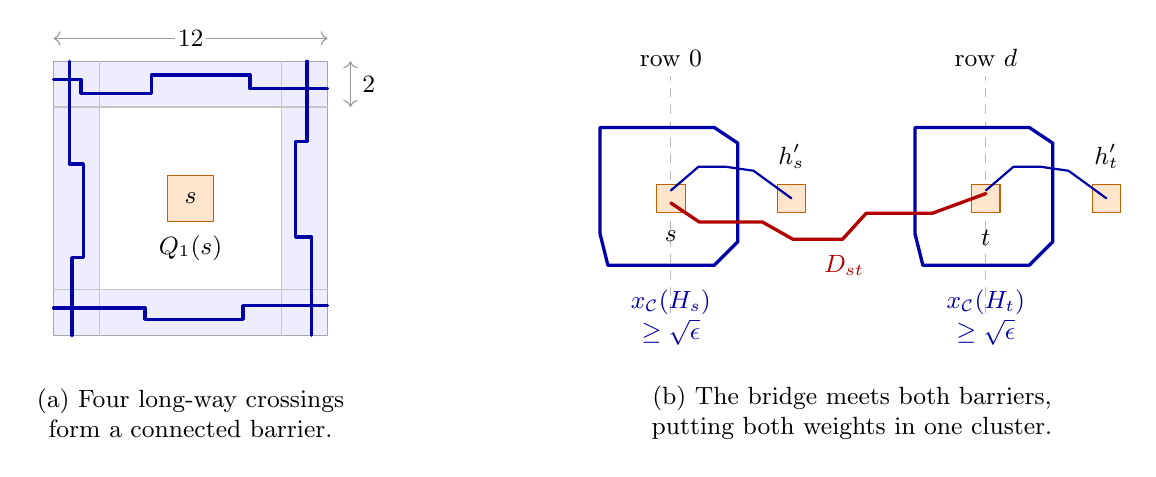
\begin{tikzpicture}[font=\small,line cap=round,line join=round]
 \begin{scope}[x=0.29cm,y=0.29cm]
  \fill[blue!7] (-6,-6) rectangle (6,6);
  \fill[white] (-4,-4) rectangle (4,4);
  \draw[gray!70] (-6,-6) rectangle (6,6);
  \draw[gray!70,dashed] (-4,-4) rectangle (4,4);
  \draw[gray!45] (-6,4)--(6,4) (-6,-4)--(6,-4)
                  (-4,-6)--(-4,6) (4,-6)--(4,6);
  \filldraw[fill=orange!20,draw=orange!75!black]
      (-1,-1) rectangle (1,1);
  \node at (0,0) {$s$};
  \node[anchor=north] at (0,-1.2) {$Q_1(s)$};
  \draw[blue!65!black,very thick]
     (-6,5.2)--(-4.8,5.2)--(-4.8,4.6)--(-1.7,4.6)
       --(-1.7,5.4)--(2.6,5.4)--(2.6,4.8)--(6,4.8);
  \draw[blue!65!black,very thick]
     (5.1,6)--(5.1,2.5)--(4.6,2.5)--(4.6,-1.7)
       --(5.3,-1.7)--(5.3,-6);
  \draw[blue!65!black,very thick]
     (6,-4.7)--(2.3,-4.7)--(2.3,-5.3)--(-2,-5.3)
       --(-2,-4.8)--(-6,-4.8);
  \draw[blue!65!black,very thick]
     (-5.2,-6)--(-5.2,-2.6)--(-4.7,-2.6)--(-4.7,1.5)
       --(-5.3,1.5)--(-5.3,6);
  \draw[<->,gray!80] (-6,7)--(6,7);
  \node[fill=white,inner sep=1pt] at (0,7) {$12$};
  \draw[<->,gray!80] (7,4)--(7,6);
  \node[anchor=west] at (7.1,5) {$2$};
  \node[align=center] at (0,-9.4)
     {(a) Four long-way crossings\\form a connected barrier.};
 \end{scope}
 \begin{scope}[shift={(6.1cm,0cm)},x=1cm,y=1cm]
  \draw[gray!55,dashed] (0,-1.45)--(0,1.55);
  \draw[gray!55,dashed] (4.0,-1.45)--(4.0,1.55);
  \node[above] at (0,1.55) {row $0$};
  \node[above] at (4,1.55) {row $d$};
  \foreach \u in {0,4} {
   \filldraw[fill=orange!20,draw=orange!75!black]
      (\u-0.18,-0.18) rectangle (\u+0.18,0.18);
   \filldraw[fill=orange!20,draw=orange!75!black]
      (\u+1.35,-0.18) rectangle (\u+1.71,0.18);
   \draw[blue!65!black,very thick]
      (\u-0.8,-0.85)--(\u+0.55,-0.85)--(\u+0.85,-0.55)
       --(\u+0.85,0.7)--(\u+0.55,0.9)--(\u-0.9,0.9)
       --(\u-0.9,-0.45)--cycle;
   \draw[blue!65!black,thick]
      (\u,0.1)--(\u+0.35,0.4)--(\u+0.7,0.4)
       --(\u+1.05,0.35)--(\u+1.53,0);
  }
  \draw[red!70!black,very thick]
    (0,-0.06)--(0.36,-0.3)--(1.16,-0.3)--(1.55,-0.52)
      --(2.18,-0.52)--(2.48,-0.19)--(3.32,-0.19)--(4,0.06);
  \node[below=3pt] at (0,-0.18) {$s$};
  \node[below=3pt] at (4,-0.18) {$t$};
  \node[above=2pt] at (1.53,0.18) {$h'_s$};
  \node[above=2pt] at (5.53,0.18) {$h'_t$};
  \node[red!70!black,below] at (2.2,-0.6) {$D_{st}$};
  \node[blue!65!black,below,align=center] at (0,-1.04)
      {$x_{\mathcal C}(H_s)$\\$\ge\sqrt\epsilon$};
  \node[blue!65!black,below,align=center] at (4,-1.04)
      {$x_{\mathcal C}(H_t)$\\$\ge\sqrt\epsilon$};
  \node[align=center] at (2.3,-2.72)
     {(b) The bridge meets both barriers,\\putting both weights in one cluster.};
 \end{scope}
\end{tikzpicture}
\caption{The geometric step in \eqref{vis:bridge}.
In (a), neighboring strip crossings meet in the corner squares.
In (b), on $A_s\cap A_t$, each barrier carries normalized weight
from the tests inside and outside it; any path in $D_{st}$ joins the
two barrier clusters.  Orange squares show test supports.  Panel (b)
is schematic: time runs horizontally and the distance between the
rings is compressed.}
\label{fig:circuits}
\end{figure}


\subsection{Taking the limits in the required order}

\begin{proof}[Proof of Proposition~\ref{vis:proposition}]
The union of the events $D_{st}$ contains
$\{0\longleftrightarrow d\}$.  Summing \eqref{vis:bridge} over the
$O(w^2)$ pairs and applying \eqref{vis:row-connection} gives
\[
 c\,e^{-(d+a)e_N(w)}
 \le\sum_{s,t}\E_{\mathrm{tor}}X_{H_s}X_{H_t}.
\]
Choose lifts with spatial center separation at most $w/2$.
The joint test supports then have spatial extent at most $w/2+O(1)$
and time extent at most $d+O(1)$, both less than $3w/4$ for large $w$.
The uniform moment comparison therefore replaces each torus
correlation by its cutoff plane value with error $Ce^{-cw}$.
For this \emph{fixed} $w$, there are only finitely many pairs of
centers, so plane moment convergence applies to all of them as
$N\to\infty$.  Their limiting correlations are bounded by
$Ce^{-m_*d}$: every pair of test supports has time separation at least
$d-O(1)$, and the kernel estimate \eqref{inp:decay} applies
to the fixed test shapes.  Consequently
\begin{equation}\label{vis:final-bound}
 \limsup_{N\to\infty}e^{-(d+a)e_N(w)}
 \le Cw^2\bigl(e^{-m_*d}+e^{-cw}\bigr).
\end{equation}

Write $L_w=\liminf_{N\to\infty}e_N(w)$.  If $L_w<\infty$, take a
subsequence on which $e_N(w)\to L_w$.  Along it $ae_N(w)\to0$, so
\eqref{vis:final-bound} yields
\[
 L_w\ge -\frac1d\log\!\left[
       Cw^2\bigl(e^{-m_*d}+e^{-cw}\bigr)\right].
\]
If $L_w=\infty$, the desired lower bound already holds.
Since $d=\lfloor\sqrt w\rfloor$, the displayed lower bound tends to
$m_*$ as $w=w_k\to\infty$, proving \eqref{vis:gap}.
\end{proof}

In particular, given $v<m_*$, every sufficiently large fixed $w_k$
satisfies $e_N(w_k)>v$ for all sufficiently large $N$, with the cutoff
threshold allowed to depend on $w_k$.  This order of quantifiers is
exactly what the finite doubling argument in
Section~\ref{sec:counting} will use.

\section{A linear bound on the low-energy state count}
\label{sec:counting}

Let $\mathcal N_{N,w}(u)$ count the transfer energies at circumference $w$
that are at most $u$, with multiplicity and including the vacuum.
The visibility estimate from Section~\ref{sec:visibility} now allows us to
turn the trace bounds into a count below the two-excitation threshold.

\begin{proposition}\label{cou:linear}
There is a constant $C$ such that, for every sufficiently large dyadic
circumference $w=w_k$,
\begin{equation}\label{cou:linear-eq}
 \limsup_{N\to\infty}\mathcal N_{N,w}(u_0)\le Cw,
 \qquad u_0=\frac32m_*.
\end{equation}
\end{proposition}

Set $u_1=13m_*/8$. The intermediate goal is the estimate
\[
 \mathcal N_{N,2w}(y)
 \le 2(1+\varepsilon_w)\mathcal N_{N,w}(y+b_w),
 \qquad u_0\le y\le u_1,
\]
with positive errors $b_w,\varepsilon_w$ summable over dyadic widths.
For each sufficiently large fixed $w$, this estimate will hold for all
sufficiently large $N$, with the cutoff threshold allowed to depend on
$w$. Summability of the energy shifts keeps the iterated threshold inside
the stated interval once the base width is large enough; the factors
$1+\varepsilon_w$ have a finite product. Thus the factor $2$ at each
doubling yields the desired linear growth in circumference.

To prove the estimate, we compare the heat trace at circumference $2w$
with the trace of two independent copies at circumference $w$. The
energies in the latter system are sums $E+E'$. If such a sum lies below
twice the gap, at least one component is the vacuum energy. A nonnegative
polynomial approximation to an energy cutoff makes this observation
quantitative without assuming convergence of individual eigenvalues.

\subsection{Exchanging time and circumference}

Rotation of the partition function gives the exact identity
\begin{equation}\label{cou:exchange}
 e^{t g_N(w)}R_{N,w}(t)
   =e^{w g_N(t)}R_{N,t}(w),
\end{equation}
where $g_N$ is the pressure correction from Section~\ref{sec:transfer}.
For a large circumference $w$, set
\[
 D=\lfloor w^{1/2}\rfloor,\qquad t_0=\lfloor D^{1/2}\rfloor.
\]
Every integer physical time is an allowed lattice length. Uniformly in the
cutoff and in the integers $t_0\le t\le D$, we claim that
\begin{equation}\label{cou:heat-product}
 \bigl|R_{N,2w}(t)-R_{N,w}(t)^2\bigr|\le Ce^{-cw}.
\end{equation}
Indeed, applying \eqref{cou:exchange} at $w$ and $2w$ yields
\begin{align*}
 \log R_{N,2w}(t)-2\log R_{N,w}(t)
  ={}&t\bigl(2g_N(w)-g_N(2w)\bigr)\\
    &+\log R_{N,t}(2w)-2\log R_{N,t}(w).
\end{align*}
The first term is exponentially small in $w$ by \eqref{tra:trace}.
The uniform positive gap at all sufficiently large circumferences,
Corollary~\ref{tra:gap}, gives a constant $c_*>0$ such that
\[
 s_{N,t}(2w)\le s_{N,t}(w)
 \le e^{-c_*(w-t)}s_{N,t}(t)\le Ce^{-c'w}.
\]
Here $s_{N,t}(t)$ is uniformly bounded by \eqref{tra:trace}.
Thus the difference of logarithms is exponentially small.
The same trace estimate bounds both $R_{N,2w}(t)$ and $R_{N,w}(t)^2$
uniformly on this time range: their logarithms are at most a polynomial
in $w$ times $e^{-ct_0}$. Exponentiating proves
\eqref{cou:heat-product}.

\subsection{A positive approximation to an energy cutoff}

For $u_0\le y\le u_1$, define
\[
 b_w=D^{-1/8},\qquad
 j_0=\left\lceil D e^{-(y+b_w/2)}\right\rceil,
 \qquad
 Q_{w,y}(x)=\sum_{j=j_0}^{D}\binom Dj x^j(1-x)^{D-j}.
\]
The polynomial is the upper tail of a binomial law, so
$0\le Q_{w,y}(x)\le1$ on $[0,1]$. Its transition occurs between energies
$y$ and $y+b_w$ when $x=e^{-E}$.

\begin{lemma}\label{cou:polynomial}
For all sufficiently large $w$, uniformly in $y\in[u_0,u_1]$,
\begin{align}
 Q_{w,y}(e^{-E})&\ge1-Ce^{-cD^{3/4}}
       &&(0\le E\le y),\label{cou:poly-low}\\
 Q_{w,y}(e^{-E})&\le Ce^{-cD^{3/4}}e^{-t_0E}
       &&(E\ge y+b_w).\label{cou:poly-high}
\end{align}
Every nonzero monomial of $Q_{w,y}$ has degree between $t_0$ and $D$,
and the sum of the absolute values of its coefficients is at most $3^D$.
\end{lemma}

\begin{proof}
The threshold $j_0/D$ differs from $e^{-y}$ and $e^{-(y+b_w)}$ by at
least $c b_w$ on their respective sides. This follows from the mean value
theorem, uniformly on the fixed energy interval, since the rounding error
is at most $1/D=o(b_w)$. Hoeffding's binomial tail bound
\cite[Theorem~1]{Hoeffding1963} therefore gives \eqref{cou:poly-low} and
\eqref{cou:poly-high} without the factor $e^{-t_0E}$, because
$Db_w^2=D^{3/4}$.

To retain a summable bound over all energies, that additional factor is
essential. Choose $c_1>0$ such that $j_0\ge c_1D$ for every allowed $y$
and all large $w$. Fix $E_*>4\log(2)/c_1+1$.
For $E\le E_*$, the loss $e^{t_0E_*}$ is absorbed by decreasing the
constant in the exponent $-cD^{3/4}$, since $t_0=O(D^{1/2})$.
For $E\ge E_*$, the binomial formula gives
\[
 Q_{w,y}(e^{-E})\le 2^D e^{-j_0E}.
\]
For large $w$, $t_0\le c_1D/2$, and consequently
\[
 2^D e^{-(j_0-t_0)E}
 \le \exp\!\left(-\frac{c_1}{4}DE\right)
 \le Ce^{-cD^{3/4}}.
\]
This proves \eqref{cou:poly-high} for every $E\ge y+b_w$.

The smallest possible degree in the expanded polynomial is $j_0$, which
is at least $t_0$ for large $w$. Finally its coefficient sum in absolute
value is bounded by
\[
 \sum_{j=j_0}^D\binom Dj 2^{D-j}\le3^D.
\]
\end{proof}

Applying \eqref{cou:heat-product} to each monomial gives
\begin{equation}\label{cou:poly-trace}
 \left|
   \sum_{E\text{ at }2w}Q_{w,y}(e^{-E})
   -\sum_{E,E'\text{ at }w}Q_{w,y}(e^{-(E+E')})
 \right|\le Ce^{-c'w}.
\end{equation}
All sums count multiplicities. They converge absolutely, since the
smallest degree is positive and the relevant heat traces are finite.
The coefficient bound costs at most $3^D$, which is absorbed by
$e^{-cw}$ because $D=O(w^{1/2})$.

\paragraph{From polynomial traces to counts.}
By the visibility estimate \eqref{vis:gap}, for each sufficiently large
fixed dyadic $w$ and all sufficiently large $N$ depending on $w$,
\[
 2e_N(w)\ge\frac74m_*.
\]
Increase the lower bound on $w$ so that $u_1+b_w<7m_*/4$. Any pair in
\eqref{cou:poly-trace} with $E+E'<y+b_w$ then has a zero component.
There are at most $2\mathcal N_{N,w}(y+b_w)$ such pairs. For the
remaining pairs, Lemma~\ref{cou:polynomial} bounds their total contribution
by
\[
 Ce^{-cD^{3/4}}\sum_{E,E'}e^{-t_0(E+E')}
 =Ce^{-cD^{3/4}}R_{N,w}(t_0)^2
 \le Ce^{-cD^{3/4}}.
\]
Using \eqref{cou:poly-low} for energies at $2w$ not exceeding $y$, and
absorbing the additive errors into $\mathcal N_{N,w}\ge1$, proves
\begin{equation}\label{cou:recursion}
 \mathcal N_{N,2w}(y)
 \le2\bigl(1+Ce^{-cD^{3/4}}\bigr)
       \mathcal N_{N,w}(y+b_w),
 \qquad u_0\le y\le u_1.
\end{equation}
The constants are independent of $N,w,y$; for each fixed $w$, the
inequality holds for all sufficiently large $N$.

\subsection{Dyadic iteration}

\begin{proof}[Proof of Proposition~\ref{cou:linear}]
Choose a fixed dyadic base width $w_{k_0}$ large enough for the preceding
estimates and so that
\[
 \sum_{k=k_0}^{\infty}b_{w_k}<u_1-u_0.
\]
This is possible because $b_{w_k}=O(w_k^{-1/16})$.
The product of the factors $1+Ce^{-c\lfloor\sqrt{w_k}\rfloor^{3/4}}$
over the same range is finite. At the base width,
\[
 \mathcal N_{N,w_{k_0}}(u_1)
 \le e^{w_{k_0}u_1}R_{N,w_{k_0}}(w_{k_0})\le C_0,
\]
uniformly in the cutoff.

Fix a target $w_k$ with $k>k_0$. Apply \eqref{cou:recursion} backwards
along the finite chain $w_k,w_{k-1},\ldots,w_{k_0}$, starting at threshold
$u_0$. The accumulated threshold shifts remain below $u_1-u_0$, so every
application is valid. For all sufficiently large $N$ on this finite
chain, we obtain
\[
 \mathcal N_{N,w_k}(u_0)
 \le C_0\,2^{k-k_0}
       \prod_{h=k_0}^{k-1}
         \left(1+Ce^{-c\lfloor\sqrt{w_h}\rfloor^{3/4}}\right)
 \le Cw_k.
\]
Taking $\limsup_{N\to\infty}$ proves the assertion. The cutoff threshold
may depend on the target width; no simultaneous limit in $N$ and $w$
has been used.
\end{proof}

\section{From the state count to an isolated mass}
\label{sec:mass-support}

Each mass in the support of $\rho$ contributes to the continuum two-point
function throughout an interval of spatial momenta. We will test these
contributions by positive measures from the finite-circumference transfer
operator. Distinct masses will then require distinct low-energy states
at every allowed momentum in that interval. Proposition~\ref{cou:linear}
bounds how many such masses there can be.

\subsection{Measures at fixed momentum}

Fix nonzero nonnegative smooth functions $g,h$ of compact support, with
$\supp g\subset(0,l)$ for a fixed positive integer $l$, and set
$f(t,b)=g(t)h(b)$. We use color $3$ throughout. On a cylinder of
circumference $w=w_k$, let $X_f$ be the source-normalized lattice field
sum and define its bounded truncation by
\[
 F=\max\{-w,\min\{X_f,w\}\}.
\]
Use the slab $[0,l]$ for the normalized insertion $A_F$, with the initial
row as its left kernel variable, and put
\[
 v=A_F\Omega_{N,w}.
\]
With this convention, the matrix element
$\langle v,T_{N,w}^{n/a}v\rangle$ places the first copy of $F$ on
$[-l,0]$ by time reflection and the second copy on $[n,n+l]$ by time
translation. To see the corresponding time weights, let $Q_{h,N}$
denote row multiplication by
$B_Na\sum_{b\in a\Z/w\Z}h(b)q_b^3$, using the periodization of $h$.
Before truncation the linear insertion satisfies the exact formula
\[
 A_{X_f}
   =a\sum_{t\in a\Z\cap[0,l]}
      g(t)T^{t/a}Q_{h,N}T^{(l-t)/a},
 \qquad
 A_{X_f}\Omega
   =a\sum_t g(t)T^{t/a}Q_{h,N}\Omega.
\]

Work in the complex transfer Hilbert space. Spatial row translations
$U_b$, for $b\in a\Z/w\Z$, commute with $T_{N,w}$. Choose their character
convention so that the momentum projection is
\[
 \Pi_p=\frac{a}{w}\sum_{b\in a\Z/w\Z}e^{-ipb}U_b,
 \qquad
 p\in\frac{2\pi}{w}\Z\cap[-\pi/a,\pi/a).
\]
For each such $p$, define the finite positive measure
\begin{equation}\label{mass:finite-measure}
 \nu_{N,w,p}
   =w\sum_E\bigl\|P_E\Pi_pv\bigr\|^2\delta_{e^{-E}}
 \quad\text{on }[0,1],
\end{equation}
where $P_E$ is the transfer-energy projection. The factor $w$ converts
the normalized character sum into a spatial Riemann sum.

Let $C_f(n,b)$ be the continuum correlation of $\phi^3(f)$ reflected in
time with a second copy translated by $n$ in time and by $b$ in space.
For a compact momentum interval $I$, we will write $\max_{p\in I}$ for
the maximum over allowed lattice momenta lying in $I$.

\begin{lemma}\label{mass:moments}
For every integer $n\ge0$ and every compact interval $I$ with nonempty
interior,
\begin{equation}\label{mass:moments-eq}
 \lim_{\substack{w\to\infty\\w=w_k}}\limsup_{N\to\infty}
 \max_{p\in I}
 \left|
   \int x^n\,\nu_{N,w,p}(dx)
   -\int_\R e^{-ipb}C_f(n,b)\,db
 \right|=0.
\end{equation}
\end{lemma}

\begin{proof}
The spectral theorem and the character formula give
\begin{align*}
 \int x^n\,\nu_{N,w,p}(dx)
 &=w\langle v,T_{N,w}^{n/a}\Pi_pv\rangle\\
 &=a\sum_{\substack{b\in a\Z\\-w/2\le b<w/2}}
       e^{-ipb}\langle v,T_{N,w}^{n/a}U_bv\rangle.
\end{align*}
The matrix element in the sum is the cylinder correlation of the two
bounded slab observables just described. For fixed $f,n$ and large $w$,
their joint support has time extent at most $n+2l$ and spatial extent at
most $w/2+\operatorname{diam}(\supp h)$. Both are below $3w/4$.
The cylinder-to-torus comparison, followed by
Proposition~\ref{tra:comparison}, replaces this correlation by its cutoff
plane counterpart with error at most $Cw^2e^{-cw}$, uniformly in $b$ and
$N$. The uniform field tails then remove the two truncations on the
plane with error $Ce^{-c'w}$, by Cauchy--Schwarz and the moment majorants.
The factor $a$ times the number of spatial translates is $w$, so the
total error in the displayed Riemann sum still tends to zero exponentially
in $w$.

For a fixed $w$, the cutoff plane smeared correlations converge uniformly
for $|b|\le w/2$ to $C_f(n,b)$. To see the uniformity, moment convergence
gives pointwise convergence, while the difference-test bound
\eqref{inp:test-difference} gives uniform equicontinuity. More explicitly,
on a fixed compact translation interval the smooth translates satisfy
$|f_b-f_{b'}|\le C|b-b'|$ on a fixed finite union of unit boxes. The
second-moment majorant bounds the $L^2$ norm of the corresponding field
difference by $C'|b-b'|$. Cauchy--Schwarz then gives the same modulus of
continuity for the correlations. Compactness upgrades pointwise
convergence to uniform convergence. Consequently, as $N\to\infty$, the
Riemann sum of the cutoff plane correlations converges to the continuum
integral over $[-w/2,w/2]$, uniformly for $p$ in $I$; the exponential
factors have a uniform modulus of continuity on this compact set.

Finally, the separated-time kernel bound in Section~\ref{sec:inputs}
implies $|C_f(n,b)|\le Ce^{-c|b|}$ outside a fixed compact interval.
The omitted spatial tail therefore tends to zero uniformly in $p$ as
$w\to\infty$. This proves \eqref{mass:moments-eq}. The case $n=0$ is
included: $\supp g$ has positive distance from zero, so the two reflected
field supports remain separated in time.
\end{proof}

The Euclidean spectral representation \eqref{inp:euclidean} identifies the
limiting measures explicitly. Write
\[
 \widehat h(p)=\int_\R e^{-ipb}h(b)\,db,
 \qquad G(E)=\int_0^l g(t)e^{-tE}\,dt,
 \qquad E(p,\mu)=\sqrt{p^2+\mu^2}.
\]
For each $p\in\R$, let $\nu_p$ be the image, under
$\mu\mapsto e^{-E(p,\mu)}$, of the positive measure
\begin{equation}\label{mass:measure}
 \frac{|\widehat h(p)|^2}{2E(p,\mu)}
       |G(E(p,\mu))|^2\,\rho(d\mu^2).
\end{equation}
Integrating the kernel against the two slab tests and then Fourier
transforming in their relative spatial displacement gives
\[
 \int_\R e^{-ipb}C_f(n,b)\,db=\int x^n\,\nu_p(dx).
\]
The time separation supplies exponential damping in $\mu$, so the
integrals converge and depend continuously on $p$ on compact intervals.
This also justifies the Fourier calculation, either directly or first
as an identity of distributions and then of continuous functions.

We will need continuous spectral tests rather than moments. For every
$\Psi\in C(I\times[0,1])$, Lemma~\ref{mass:moments} implies
\begin{equation}\label{mass:continuous-tests}
 \lim_{\substack{w\to\infty\\w=w_k}}\limsup_{N\to\infty}
 \max_{p\in I}
 \left|
  \int\Psi(p,x)\,\nu_{N,w,p}(dx)
   -\int\Psi(p,x)\,\nu_p(dx)
 \right|=0.
\end{equation}
Indeed, the $n=0$ case uniformly bounds the total masses in this iterated
limit. Approximate $\Psi$ uniformly by polynomials in $x$ with continuous
coefficients in $p$, for instance its Bernstein polynomials in $x$.
Each coefficient is bounded on $I$, so Lemma~\ref{mass:moments} applies
to the finite sum; the uniform approximation controls the remainder
against both measures. Thus no mass near $x=0$ is lost in passing from
moments to continuous tests.

\subsection{Finiteness of the low mass support}

\begin{proposition}\label{mass:finite-support}
The set
\[
 \{\mu\in[m_*,5m_*/4]:\mu^2\in\supp\rho\}
\]
is finite.
\end{proposition}

\begin{proof}
Choose $p_0>0$ so small that
\[
 \sqrt{p_0^2+(5m_*/4)^2}<u_0,
 \qquad \widehat h(p)\ne0\quad (|p|\le p_0).
\]
This is possible because $5m_*/4<u_0=3m_*/2$ and
$\widehat h(0)=\int h>0$. This momentum interval is fixed before any
finite collection of masses is selected.

Choose $J$ distinct masses $\mu_1,\ldots,\mu_J$ from the indicated
support. On $I=[-p_0,p_0]$, the curves
\[
 x_j(p)=e^{-E(p,\mu_j)},\qquad j=1,\ldots,J,
\]
are pairwise disjoint compact graphs in $I\times(e^{-u_0},1)$. Their
mutual distances and their distances from the two horizontal boundary
lines are positive. There are therefore nonnegative continuous functions
$\Psi_j$ on $I\times[0,1]$, supported in mutually disjoint neighborhoods
of these graphs contained in $I\times(e^{-u_0},1)$, and equal to one on
the respective graphs.

For every $p\in I$,
\[
 L_j(p):=\int\Psi_j(p,x)\,\nu_p(dx)>0.
\]
Indeed, membership of $\mu_j^2$ in $\supp\rho$ gives positive measure to
every neighborhood of that point. The integrand in \eqref{mass:measure}
is positive there: $\widehat h(p)\ne0$ and $G(E)>0$ for every $E>0$,
since $g\ge0$ is nonzero. Continuity of $\Psi_j$ makes its value positive
through a neighborhood of $\mu_j$ at the fixed momentum. Moreover
$L_j$ is continuous in $p$, by exponential domination in
\eqref{mass:measure}. Compactness yields
\[
 \eta:=\min_{1\le j\le J}\min_{p\in I}L_j(p)>0.
\]
Both $\eta$ and the required approximation scale may depend on this
finite collection of masses.

By \eqref{mass:continuous-tests}, for all sufficiently large fixed
dyadic $w$, and then all sufficiently large $N$ depending on $w$,
\[
 \int\Psi_j(p,x)\,\nu_{N,w,p}(dx)>\eta/2
 \qquad (j=1,\ldots,J)
\]
at every allowed $p\in I$. Each atom of the measure
\eqref{mass:finite-measure} comes from a transfer-energy eigenspace
with momentum $p$. The disjoint
supports of the $\Psi_j$ therefore require at least $J$ distinct energies
below $u_0$ in that space. Distinct momentum spaces are orthogonal.
For large $w$, the number of momenta in $I$ is at least
$c_0w$, where $c_0>0$ depends only on $p_0$; at any fixed $w$ these are
distinct Brillouin characters once $N$ is large. Thus
\[
 Jc_0w\le\mathcal N_{N,w}(u_0).
\]
Taking the cutoff limit and using Proposition~\ref{cou:linear} gives
$Jc_0\le C$. The constants $c_0,C$ are independent of the selected
masses and of $J$. The support can consequently contain only finitely
many points in the stated interval.
\end{proof}

\begin{proof}[Proof of Theorem~\ref{intro:main}]
The nonempty closed mass support has minimum $m_*>0$, by the continuum
inputs in Section~\ref{sec:inputs}. Proposition~\ref{mass:finite-support}
makes this minimum isolated in the support. A positive locally finite
measure assigns strictly positive finite mass to an isolated support
point, so
\[
 Z=\rho(\{m_*^2\})\in(0,\infty).
\]
Choose $\delta>0$ small enough that no other mass in the support lies
below $m_*+\delta$, and define
\[
 m_1=m_*,\qquad \rho_{\mathrm{rest}}=\rho-Z\delta_{m_*^2}.
\]
This is a positive measure, and its support is contained in
$[(m_1+\delta)^2,\infty)$, as required.
\end{proof}

\bibliographystyle{plain}
\bibliography{references}
\end{document}
